\indent This experiment was part of a group of four experiments that commissioned the new Hall C Super High Momentum Spectrometer (SHMS) as part of the 12 GeV upgrade at JLab.
An electron beam was incident on a 10 cm long liquid deuterium target (LD2). The scattered electron and knocked-out proton were detected in coincidence
by the SHMS ans High Momentum Spectrometer (HMS), respectivly. The ``missing'' (undetected) neutron was reconstructed from momentum conservation laws.
The beam currents delivered by the accelerator ranged between 40-60 $\mu$A due to frequent beam trips at higher currents and the beam was rastered over a 2x2 mm$^{2}$ area to reduce
the effects of localized boiling on the cryogenic targets (hydrogen and deuterium). \\
\indent Both spectrometers at Hall C have similar standard detector packages, each with 1) four sets of hodoscope planes (scintillator arrays) used for triggering,
2) a pair of drift chambers used for tracking, 3) a calorimeter used for $e^{-}/\pi^{-}$ discrimination and 4) a gas \u{C}erenkov used also for $e^{-}/\pi^{-}$ and an additional
Noble Gas \u{C}erenkov used in the SHMS for $e^{-}/\pi^{+}/K^{+}$ at momenta $>$ 6 GeV/c. Due to the absence of significant background on this experiment and the low coincidence trigger rates
($\sim 1-3$ Hz) at the higher missing momentum settings, the use of additional particle identification (PID) was found to have little to no effect on the final cross section. \\
\indent We measured three missing momentum settings: $p_{r}=80,580$ and $750$ MeV/c. In the high missing momentum settings the spectrometer configuration was changed
multiple times resulting in either the spectrometer angle or momentum not being excactly the same. As a result, two separate data sets measured for the 580 MeV/c and three data sets for the 750 MeV/c setting.  
The spectrometer central settings are approximately as follows: the SHMS central angle and momentum settings were kept fixed at (12.194 deg, 8.5342 GeV/c) and the HMS central angle and momentum settings were changed from
(38.896 deg, 2.840 GeV/c) at the 80 MeV setting to (54.992 deg, 2.1925 GeV/c) and (58.391 deg, 2.0915 GeV/c) at the 580 and 750 MeV/c settings, respectively. At these kinematics, the
3-momentum transfer is $|\vec{q}| = 2.86$ GeV/c and is on the order of the final proton momentum indicating that most of the energy and momentum are transferred to the proton. As a result, the ejected proton
scatters at angles $\theta_{pq}\sim 0$, relative to the $\vec{q}$. This configuration is known as the ``parallel-kinematics'' and suppresses the process in which the neutron is struck and the proton is a spectator. \\
\indent In addition to deuteron kinematics,  $^{1}H(e,e'p)$ elastic data was also taken at kinematics close to the deuteron 80 MeV setting for cross-checks with the spectrometer acceptance model as well as for normalization purposes using the  Hall C Monte Carlo
simulation program, \texttt{SIMC}. Additional $^{1}H(e,e'p)$ data was also taken at three other kinematic settings that covered the entire SHMS momentum acceptance range and were used for spectrometer optics studies and
calibration. \\
\indent The event selection criteria for the hydrogen and deuteron data was determined by making 1) standard cuts on the spectrometer momentum fraction ($\delta$) to select a region in which the reconstruction optics
is well known, 2) an HMS collimator cut to restrict the spectrometer solid angle acceptance to events that only passed through the collimator and not by re-scattering from the edges, 3) a missing
energy cut (peak $\sim$ 2.2 MeV for the deuteron) to select true $ep$ coincidences and not events from the radiative tail, 4) a coincidence time cut to select true coincidence events and not accidentals,  5) a PID cut on the
SHMS calorimeter to select electrons and not other sources of background, mostly pions and 6) a z-vertex difference cut between the HMS and SHMS $z$ reaction vertex difference to select events that truly
originated from the same reaction vertex at the target. \\
\indent The experimental data yield was normalized by the accumulated charge and corrected for tracking efficiencies, total live time, proton absorption and target boiling factors.
For $^{1}H(e,e'p)$, the corrected data yield was compared against SIMC using P. Bosted's proton form factor parametrization\cite{PhysRevC.51.409} to check the spectrometer acceptance
model. The data to SIMC yield ratio was determined to be 1.0 within uncertainty, and there was no need to include an overall hydrogen normalization factor. For the $^{2}H(e,e'p)$ data,
the theoretical cross section calculation from J.M. Laget using the Paris potential was incorporated into SIMC as a subroutine. The events generated
over phase space were weighted by the theoretical cross sections using either the PWIA or FSI models and were compared to the corrected data yield for the 80 MeV setting. Variations
of up to $\sim 20 \%$ for recoil momentum up to $\sim$ 250 MeV/c were observed which are typical for this setting. The 80 MeV data was also checked for reproducibility against the Hall A data
at this setting. This agreement gives us confidence on the measurements made at higher missing momentum setting for which no data exists. \\
\indent The experimental sections were determined by dividing the normalized data yield by the phase space over the spectrometers acceptances generated in SIMC. The data was radiatively corrected
by multiplying measured cross sections by the ratio of the SIMC yield (using the Paris potential, FSI model) without and with radiative effects for each bin in ($\theta_{nq}, p_{r}$).
The data was also bin-centered corrected by multiplying the radiative corrected cross sections by the ratio of theoretical cross section at the averaged kinematics to the average SIMC model
cross sections at the bin-centered value in ($\theta_{nq}, p_{r}$). The theoretical cross sections were determined external to SIMC using J.M. Laget's calculations at the averaged kinematics.\\
\begin{figure}
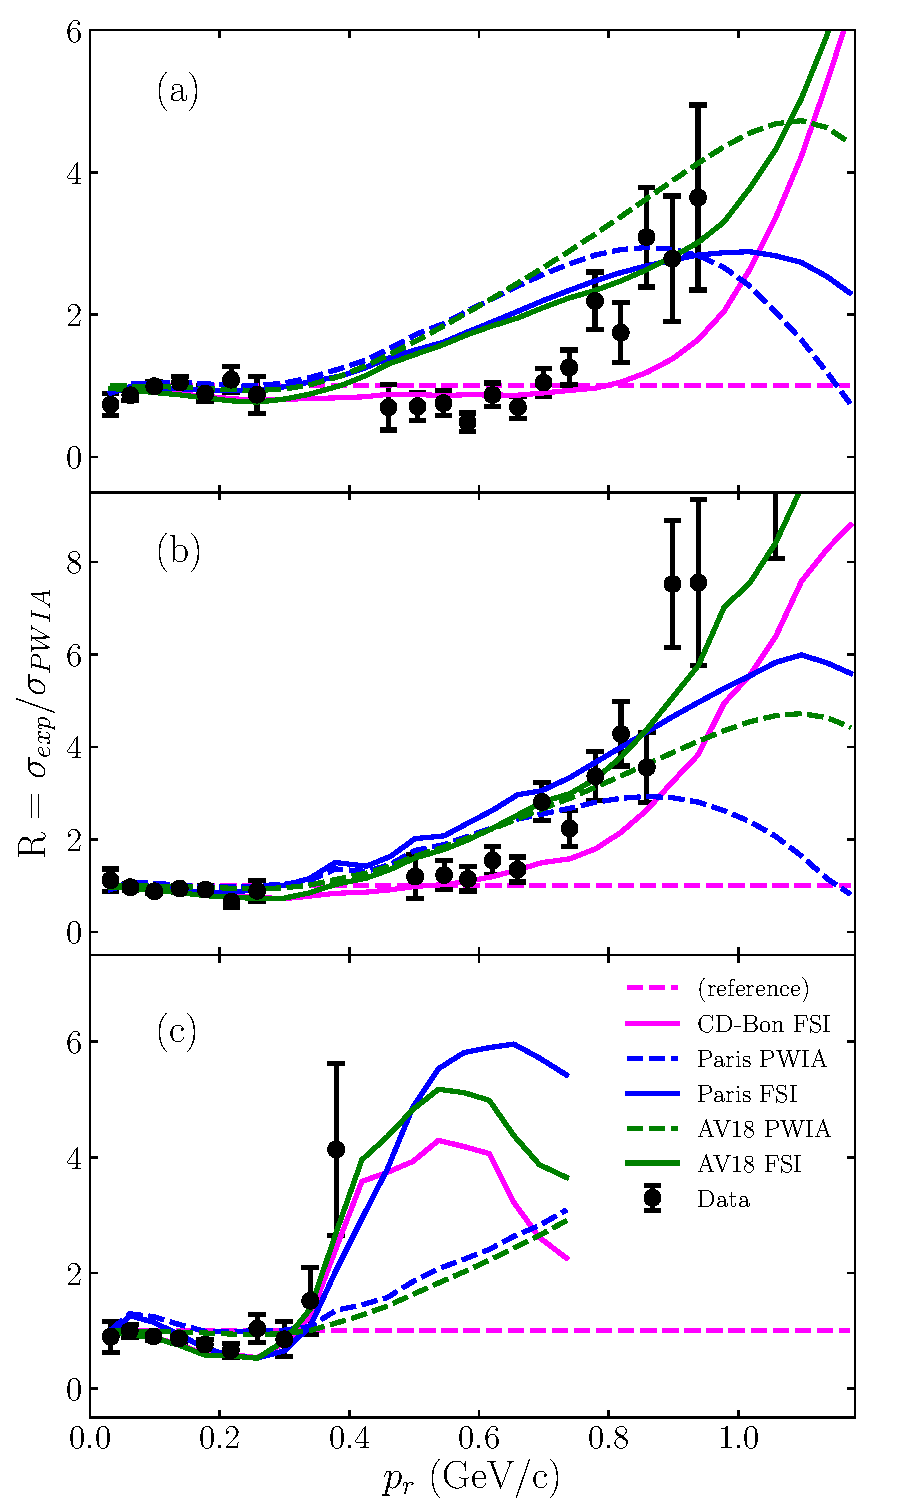
\includegraphics[scale=0.5]{prl_plots/PRL_plot2.pdf}
\caption{\label{fig:fig1} The ratio R($p_{r}$) = $\sigma_{exp}/\sigma_{PWIA}$ is shown in (a)-(c) for $\theta_{nq}=35^{o}, 45^{o}$ and $75^{o}$, respectively, each with a bin width of $\pm 5^{o}$.
                          The dashed reference (magenta) line refers to CD-Bonn PWIA for which the data and all models are divided. }
\end{figure}
\indent The systematic uncertainties on the measured cross sections are separated in two categories: 1) normalization and 2) kinematic uncertainties. The normalization uncertainties on
the  $^{2}H(e,e'p)n$ cross section were determined to be: tracking efficiencies ($0.40 \%$-HMS, $0.59 \%$-SHMS ), target boiling ($0.39 \%$), total live time ($3.0 \%$) and total charge ($2.0\%$)
for an overall normalization uncertainty of $3.7 \%$ added in quadrature. \\
\indent The kinematic uncertainties were determined point-to-point for ($\theta_{nq}, p_{r}$) bins for each data set independently, and added in quadrature for overlapping $p_{r}$ bins
of different data sets. The variations of the cross section with spectrometer kinematics in beam energy, electron angle and momentum and proton angle were determined from Laget PWIA model and the uncertainties
in the kinematic variables were determined from a fit to the $^{1}H(e,e'p)$ elastic data.
%For $\theta_{nq}=$ 35, 45 and 75 deg the overall kinematic uncertainty varied up to 6.5$\%$ for $p_{r}\leq1.01$ GeV/c.
The overall systematic uncertainty in the cross section was determined by the quadrature sum of the normalization and kinematic uncertainties. This results was then added in quadrature
to the statiscial uncertainty to obtain the final uncertainty in the cross section. \\
\indent The $^{2}H(e,e'p)n$ reduced cross sections for each data set were determined within the PWIA by:
\begin{equation}
\sigma_{red} \equiv \frac{\sigma_{exp}}{Kf_{rec}\sigma_{cc1}}
\label{eq:1}
\end{equation}
where $\sigma_{exp}$ is the 5-fold experimental (or model) cross section, $K$ is a kinematical factor, $f_{rec}$ is a the recoil factor that arises from the
integration over missing energy and $\sigma_{cc1}$ is the de Forest\cite{DEFOREST1983} electron-proton offshell cross section.
In the PWIA, $\sigma_{red}$ is interpreted as the momentum distributions inside the deuteron where most of the kinematical dependencies that arise from the
cross section have been factored out. \\
\indent In Figure \ref{fig:fig1}, the ratio of the experimental to the PWIA reduced cross sections is plotted against neutron recoil momentum, $p_{r}$. 

